%; whizzy chapter
% -initex iniptex -latex platex -format platex -bibtex jbibtex -fmt fmt
% $B0J>e(B whizzytex $B$r;HMQ$9$k>l9g$N@_Dj!#(B


%     Tokyo Debian Meeting resources
%     Copyright (C) 2009 Junichi Uekawa

%     This program is free software; you can redistribute it and/or modify
%     it under the terms of the GNU General Public License as published by
%     the Free Software Foundation; either version 2 of the License, or
%     (at your option) any later version.

%     This program is distributed in the hope that it will be useful,
%     but WITHOUT ANY WARRANTY; without even the implied warranty of
%     MERCHANTABILITY or FITNESS FOR A PARTICULAR PURPOSE.  See the
%     GNU General Public License for more details.

%     You should have received a copy of the GNU General Public License
%     along with this program; if not, write to the Free Software
%     Foundation, Inc., 51 Franklin St, Fifth Floor, Boston, MA  02110-1301 USA

%  preview (shell-command (concat "evince " (replace-regexp-in-string "tex$" "pdf"(buffer-file-name)) "&"))
% $B2hA|%U%!%$%k$r=hM}$9$k$?$a$K$O(Bebb$B$rMxMQ$7$F(Bboundingbox$B$r:n@.!#(B
%(shell-command "cd image200901; ebb *.png")

%%$B$3$3$+$i%X%C%@3+;O!#(B

\documentclass[mingoth,a4paper]{jsarticle}
\usepackage{monthlyreport}

% $BF|IU$rDj5A$9$k!"Kh7nJQ$o$j$^$9!#(B
\newcommand{\debmtgyear}{2009}
\newcommand{\debmtgmonth}{3}
\newcommand{\debmtgdate}{21}
\newcommand{\debmtgnumber}{50}



\begin{document}

\begin{titlepage}
\thispagestyle{empty}

% $B%?%$%H%k%Z!<%8(B:$BJT=8I,MW$JItJ,$O:G=i$N%^%/%m$KHt$P$9$3$H(B

\vspace*{-2cm}
$BBh(B\debmtgnumber{}$B2s(B $BEl5~%(%j%"(B Debian $BJY6/2q;qNA(B

\hspace*{-2.4cm}
\includegraphics[width=210mm]{image200801/2008title.eps}\\
\hfill{}\debmtgyear{}$BG/(B\debmtgmonth{}$B7n(B\debmtgdate{}$BF|(B

\end{titlepage}

\dancersection{Introduction}{$B>e@n(B $B=c0l(B}

\begin{multicols}{2}
 
 
 $B:#7n$N(BDebian$BJY6/2q$X$h$&$3$=!#$3$l$+$i(BDebian$B$N@$3&$K$"$7$rF'$_F~$l$k$H(B
 $B$$$&J}$b!"$9$G$K$I$C$W$j$H$D$+$C$F$$$k$H$$$&J}$b!"7n$K0l2s(BDebian$B$K$D$$(B
 $B$F8l$j$^$;$s$+!)(B

 Debian$BJY6/2q$NL\E*$O2<5-$G$9!#(B

 \begin{itemize}
 \item \underline{Debian Developer} ($B3+H/<T(B)$B$N0i@.!#(B
 \item $BF|K\8l$G$N!V(B\underline{$B3+H/$K4X$9$k>pJs(B}$B!W$r@0M}$7$F$^$H$a!"%"%C%W%G!<%H$9$k!#(B
 \item \underline{$B>l(B}$B$NDs6!!#(B
 \begin{itemize}
  \item $BIaCJ$P$i$P$i$J>l=j$K$$$k?M!9$,(B face-to-face $B$G=P2q$($k>l$rDs6!(B
	$B$9$k!#(B
  \item Debian $B$N$?$a$K$J$k$3$H$r8l$k>l$rDs6!$9$k!#(B
  \item Debian$B$K$D$$$F8l$k>l$rDs6!$9$k!#(B
 \end{itemize}
 \end{itemize}		

 Debian$B$NJY6/2q$H$$$&$3$H$G5f6KE*$K$O;22C<TA40w$,(BDebian Package$B$r$,$j$,$j(B
 $B$H:n$k%9!<%Q!<%O%C%+!<$K$J$C$?;Q$rLQA[$7$F$$$^$9!#>pJs$N6&M-!&3hMQ$rDL$7(B
 $B$F(B Debian$B$N:#8e$NG=F0E*$JE83+$X$NEZBf$H$7$F!"!V>l!W$H$7$F$N6u4V$rDs6!$9(B
 $B$k$N$,L\E*$G$9!#(B

 2009$BG/$N7W2h$O2>$G$9!#(B

 \begin{enumerate}
  \item $B?7G/$N4k2h(B ($B%"%s%5%s%V%k2.7&3+:E(B)
  \item OSC
  \item ($BEl5~Bg3X(B?)
  \item ($B@iBeED6hETN)?^=q4[(B?\footnote{\url{http://www.library.chiyoda.tokyo.jp/}})
  \item ($BEl5~Bg3X(B?)
  \item 
  \item $B%9%Z%$%s$K$F3+:E(B
  \item Debconf$BJs9p2q(B
  \item 
  \item 
  \item 
  \item $BK:G/2q(B
 \end{enumerate}

 $B2q>l8uJd$H$7$F$O2<5-$,$"$j$^$9(B:

 \begin{itemize}
  \item $BBg3X(B
  \item $B7CHf<w(BSGI$B%[!<%k(B
  \item Google$B%*%U%#%9(B
  \item $B8xL14[(B($B$"$s$5$s$V$k2.7&Ey(B)
  \item $BETN)2q5D<<(B($BL5@~(BLAN)
  \item $B7rJ]$N;\@_(B
 \end{itemize}

\end{multicols}


\newpage

\begin{minipage}[b]{0.2\hsize}
 \definecolor{titleback}{gray}{0.9}
 \colorbox{titleback}{\rotatebox{90}{\fontsize{80}{80} {\gt $B%G%S%"%sJY6/2q(B} }}
\end{minipage}
\begin{minipage}[b]{0.8\hsize}
\hrule
\vspace{2mm}
\hrule
%
% there are too many entries in 200901, usually
% we have tocdepth=2.
%
\setcounter{tocdepth}{1}
\tableofcontents
\vspace{2mm}
\hrule
\end{minipage}

\dancersection{$B;vA02]Bj(B}{$B>e@n(B $B=c0l(B}

??

{\bf $BLdBj(B}

\begin{enumerate}
 \item xxx
\end{enumerate}

$B$3$N2]Bj$KBP$7$FDs=P$$$?$@$$$?FbMF$O0J2<$G$9!#(B

\begin{multicols}{2}
%; whizzy-master ../debianmeetingresume200901.tex
% $B0J>e$N@_Dj$r$7$F$$$k$?$a!"$3$N%U%!%$%k$G(B M-x whizzytex $B$9$k$H!"(Bwhizzytex$B$,MxMQ$G$-$^$9!#(B

\begin{prework}{$B>e@n=c0l(B}
\preworksection{XXXX}

\end{prework}

% $B$3$N>e$NItJ,$K0J2<$NFbMF$rA^F~$9$k!#(B
% \begin{prework}{$BL>A0(B}
% \preworksection{XXX}
% \preworksection{YYY}
% \end{prework}
%

\end{multicols}

% image200903/prework.tex $BFbIt$K%F%-%9%H$rDI2C$7$F$/$@$5$$!#(B
%
%

\dancersection{$B:G6a$N(BDebian$B4XO"$N%_!<%F%#%s%0Js9p(B}{$B>e@n(B $B=c0l(B}
\subsection{$BEl5~%(%j%"(BDebian$BJY6/2q(B48$B2sL\Js9p(B}
% (query-replace-regexp "<.*?>" "")
% (query-replace-regexp "^[	 ]\+" "")

\subsection{$BEl5~%(%j%"(BDebian$BJY6/2q(B49$B2sL\Js9p(B}
% (query-replace-regexp "<.*?>" "")
% (query-replace-regexp "^[	 ]\+" "")


\subsection{Ubuntu XXX}

$B$d$^$M$5$s$,=q$/(B?



% ===============================================================
\dancersection{$B%+!<%M%kFI=q2q!!%G%#%9%H%j%S%e!<%7%g%sBg=89g(B}{$B>e@n=c0l(B}
\index{kernel}
\index{SVM}
\index{distribution}
\index{$B$V$s$5$s(B@$BJ,;6(B}
% ===============================================================

%============================================================
\dancersection{advi$B$r%G%P%C%0$7$F$_$?(B}{$BF|HfLn(B $B7<(B}
\index{OCaml}
\index{TeX}
%============================================================

11$B7n$N(BLaTeX$B$r;H$C$?%O%s%:%*%s$G!"(Bwizzytex-mode$B$+$i;H$o$l$F$$$k(B
advi$B$,$H$-$I$-8G$^$C$F$7$^$&LdBj$K$D$$$FD4$Y$F$_$^$7$?!#(B

\subsection{advi$B$,$^$k(B?}

advi$B$O0l8+IaDL$N(BDVI viewer$B$J$N$G$9$,!"$J$<$+(BOCaml$B$H$$$&JQ$o$C$?8@8l$G<BAu$5$l$F$$$^$9!#(B
$B:#2s$O(Badvi$B$+$i8F$P$l$k(Bghostscript$B$,;_$^$C$F$$$k$i$7$$!"(B
$B$H$$$&$3$H$^$GJ,$+$C$F$$$k>uBV$+$iD4$Y;O$a$^$7$?!#(B

\subsection{$B$H$j$"$($:%"%?%j$r$D$1$k(B}

$B$H$j$"$($:!"LdBj$,5/$-$F$$$k%=!<%9$r<h$C$F$-$FE83+$7$F$_$^$9!#(B

\begin{commandline}
% apt-get  source advi
...
dpkg-source: extracting advi in advi-1.6.0
dpkg-source: info: unpacking advi_1.6.0.orig.tar.gz
dpkg-source: info: applying advi_1.6.0-13.diff.gz
% cd advi-1.6.0
% ls *.ml
addons.ml     drawimage.ml  font.ml            gs.ml             main.ml     search.ml      transimpl.ml
ageometry.ml  driver.ml     global_options.ml  gterm.ml          misc.ml     shot.ml        ttfont.ml
...
\end{commandline}

*.ml$B$H$$$&$N$,(BOCaml$B$N%=!<%9%U%!%$%k$G$9!#$J$s$+!"(Bgs.ml$B$H$+$$$&$=$N$b$N%:%P%j$C$]$$$b$N$,8+$($^$9!#(B
gs.ml$B$NCf$r$^$:(Bgs$B$G8!:w$7$F$$$C$F$_$k$H!"(B

\begin{commandline}
...
  let command = Config.gs_path in
  let command_args =
    [|
      command; 
      "-dNOPLATFONTS"; "-dNOPAUSE";
      "-sDEVICE=" ^ (if !antialias then x11alpha else x11);
      "-q";
      "-dSAFER";
      "-";
    |] in

  let _ = debugs command;
...
\end{commandline}

$B$*$*!"$=$l$C$]$$!#$"$H!"%G%P%C%0MQ$C$]$$5!G=(B - debugs $B$rH/8+!#(B
$B$5$i$K$3$s$I$O(Bcommand$B$GC5$7$F$$$/$H!"(B

\begin{commandline}
...
  let lpd_in, lpd_out = Unix.pipe () in
...
  let leftout = Unix.out_channel_of_descr lpd_out in
...
  let pid =
    Unix.create_process command command_args lpd_in rpd_out
      (* Unix.stdout *) Unix.stderr
...
    method line l =
      try
        showps l;
        output_string leftout l;
        output_char leftout '\n';
...
\end{commandline}

$B$I$&$d$i(Bgs$B$K%Q%$%W$G(BPS$B$r=q$-$3$s$G$$$k$h$&$G$9!#(B
showps $B$H$+$$$&$N$G(BPS$B$NCf?H$r8+$k$3$H$,$G$-$k$s$8$c$J$$$+$J!<$H$+!#(B

\subsection{$B$^$8$a$KD4$Y$F$_$?$s$G$9$,(B...}

$B$b$&0lEY!"$3$s$I$O(Bgs.ml$B$N:G=i$NJ}$+$i%G%P%C%0MQ$N5!G=$@$18+$F$$$-$^$9!#(B

\begin{commandline}
...
let debugs = Misc.debug_endline;;
...
let showps_ref = ref false;;
let showps s =
  if !showps_ref then (print_endline  (Printf.sprintf "%s" s));;
...
Options.add
  "--showps" (Arg.Set showps_ref)
  "  ask advi to print to stdout a copy\
  \n\t of the PostScript program sent to gs.";;
...
\end{commandline}

\verb|Misc.| $B$H$$$&$N$O(B Misc$B$H$$$&JL$N%b%8%e!<%k$X$N;2>H$G$9!#$3$3$G$OC1$K(Bmisc.ml$B$NCf$r8+$l$P$h$5$=$&$G$9!#(B
\verb|showps_ref|$B$O=q$-49$(2DG=$J%U%i%0$N$h$&$G$9!#(B
$B$H;W$C$?$i$9$02<$K%3%^%s%I%i%$%s0z?t$+$i%U%i%0$r%;%C%H$G$-$k$h$&$K$J$C$F$$$k$h$&$G$9!#(B
misc.ml$B$NCf$b8+$F$_$k$H!"(B

\begin{commandline}
...
(* Debugging. *)
let forward_debug_endline =
  ref (function (_ : string) -> failwith "undefined forward debug_endline");;

let debug_endline s = (!forward_debug_endline s : unit);;

let set_forward_debug_endline f = forward_debug_endline := f;;
...
\end{commandline}

$B$5$i$K(B\verb|set_forward_debug_endline|$B$G(Bgrep$B$9$k$H!"(B\verb|global_options.ml|$B$,0z$C$+$+$k$N$G!"$=$NCf$b8+$F$_$k$H(B

\begin{commandline}
...
(* To print debugging messages. *)
let debug_endline = Options.debug "--debug" " General debug";;

(* Setting the forward in Misc. *)
Misc.set_forward_debug_endline debug_endline;;
...
\end{commandline}

$B7k6I!"$I$C$A$b%3%^%s%I%i%$%s$+$i@_Dj$G$-$k$h$&$G$9$M!#(B
$B$5$C$=$/;n$7$F$_$k$H!"(B

\begin{commandline}
% platex debianmeetingresume200812-presentation.tex
...
% advi debianmeetingresume200812-presentation.dvi
...
/usr/bin/gs
-dNOPLATFONTS
-dNOPAUSE
-sDEVICE=x11
-q
-dDELAYSAFER
-
...
%!PS-Adobe-2.0
%%Creator: Active-DVI
%!
[1 0 0 -1 0 0] concat
(/usr/share/texmf-texlive/dvips/base/texc.pro) run
(/usr/share/texmf-texlive/dvips/base/special.pro) run
...
%% Newpage

grestore
0 0 moveto
TeXDict begin 12769384 12769384 div dup /Resolution X /VResolution X end
TeXDict begin /DVImag 194.845342 def end
gsave
flushpage (...
) print flush 
\end{commandline}

$B$?$7$+$K(Bgs$B$N%3%^%s%I%i%$%s$i$7$-$b$N$H!"$=$l$+$i=q$-$3$s$@(BPS$B$NFbMF$i$7$$$b$N$,8+$($F$^$9!#(B
PS$B$GL\0u$H$J$kJ8;zNs$r=PNO$5$l$kL?Na(B \verb|flushpage (...) print flush| $B$r(Bgs$B$K=q$-$3$s$G!"(B
$B$=$N=PNO$rBT$C$F$$$k$h$&$J$N$G$9$,!"La$C$F$-$F$$$J$$$h$&$G$9!#(B

gs$B$,;_$^$C$F$7$^$&>l9g$H$=$&$G$J$$>l9g$bHf$Y$F$_$?$N$G$9$,!"(B
$B;_$^$C$F$7$^$&>l9g$N(BPS$B$N:G>.%;%C%H$r3d$j=P$9$N$,Fq$7$/!"$h$/$o$+$j$^$;$s$G$7$?!#(B

\subsection{$BJL$N2sHr:v(B?}

$B$J$K$+JL$NJ}K!$G;_$^$C$F$7$^$&$N$r2sHr$G$-$J$$$+!"$H(Bgs$B$N=PNO$rBT$C$F$$$kItJ,$b8+$F$_$^$9!#(B

\begin{commandline}
...
let rec select fd_in fd_out fd_exn timeout =
  (* dirty hack: Graphics uses itimer internally! *)
  let start = Unix.gettimeofday () in
  try
    Unix.select fd_in fd_out fd_exn timeout
  with
    Unix.Unix_error (Unix.EINTR, _, _) as exn ->
      let now = Unix.gettimeofday () in
      let remaining = start +. timeout -. now in
      if remaining > 0.0 then select fd_in fd_out fd_exn timeout else [], [], []
...
      match select [ rpd_in ] [] [] 1.0 with
      | [], _, _ ->
          begin match Unix.waitpid [ Unix.WNOHANG ] pid with
          | x, Unix.WEXITED y when x > 0 ->
              raise (Killed "gs exited")
          | 0, _ ->
              raise (Killed "gs alive but not responding")
          | _, _ ->
              raise (Killed "gs in strange state")
          end
...
\end{commandline}

gs$B$N=PNO$r(Bselect$B$GBT$C$F$$$k$h$&$G$9!#%?%$%`%"%&%H$b;E9~$s$G$"$k$h$&$G$9!#(B
$B$J$<$&$^$/$$$C$F$$$J$$$N$G$7$g$&!#(B

$B$3$3$G$OA0H>$GDj5A$5$l$F$$$k(Bselect$B$KCmL\$G$9!#(B
$B$;$C$+$/%?%$%`%"%&%H$N;D$j;~4V$r7W;;$7$F$$$k$N$K!"EO$7$F$$$k$N$O$b$H$NCM$G$9!#(B
$B$I$&$j$G$$$D$^$G$?$C$F$b%?%$%`%"%&%H$7$J$$$o$1$G$9!#(B

\begin{commandline}
...
if remaining > 0.0 then select fd_in fd_out fd_exn timeout else [], [], []
...
\end{commandline}

$B$3$l$r(B
\begin{commandline}
...
if remaining > 0.0 then select fd_in fd_out fd_exn remaining else [], [], []
...
\end{commandline}

$B$HD>$9$H!"(Bgs$B$rBT$C$F$b%?%$%`%"%&%H$9$k$h$&$K$J$j$^$9!#(B
gs$B$,8G$^$k860x$r<h$j=|$/$h$&$J:,K\E*$J2r7h$O$G$-$^$;$s$G$7$?$,!"(B
$B$H$j$"$($:$O(B advi $B$,;_$^$i$J$$$h$&$K$O$J$j$=$&$G$9!#(B


\clearpage

%\printindex

\cleartooddpage

\vspace*{15cm}
\hrule
\vspace{2mm}

\includegraphics[width=2cm]{image200502/openlogo-nd.eps}
\noindent \Large \bf Debian $BJY6/2q;qNA(B\\ \\
\noindent \normalfont \debmtgyear{}$BG/(B\debmtgmonth{}$B7n(B\debmtgdate{}$BF|(B \hspace{5mm}  $B=iHGBh(B1$B:~H/9T(B\\
\noindent \normalfont $BEl5~%(%j%"(B Debian $BJY6/2q(B $B!JJT=8!&0u:~!&H/9T!K(B\\
\hrule


\end{document}
